\documentclass[a4paper, man, floatsintext]{apa6}
\usepackage{lmodern}
\usepackage{amssymb,amsmath}
\usepackage{ifxetex,ifluatex}
\usepackage{fixltx2e} % provides \textsubscript
\ifnum 0\ifxetex 1\fi\ifluatex 1\fi=0 % if pdftex
  \usepackage[T1]{fontenc}
  \usepackage[utf8]{inputenc}
\else % if luatex or xelatex
  \ifxetex
    \usepackage{mathspec}
  \else
    \usepackage{fontspec}
  \fi
  \defaultfontfeatures{Ligatures=TeX,Scale=MatchLowercase}
\fi
% use upquote if available, for straight quotes in verbatim environments
\IfFileExists{upquote.sty}{\usepackage{upquote}}{}
% use microtype if available
\IfFileExists{microtype.sty}{%
\usepackage{microtype}
\UseMicrotypeSet[protrusion]{basicmath} % disable protrusion for tt fonts
}{}
\usepackage{hyperref}
\hypersetup{unicode=true,
            pdfauthor={Jana B. Jarecki},
            pdfborder={0 0 0},
            breaklinks=true}
\urlstyle{same}  % don't use monospace font for urls
\usepackage{graphicx,grffile}
\makeatletter
\def\maxwidth{\ifdim\Gin@nat@width>\linewidth\linewidth\else\Gin@nat@width\fi}
\def\maxheight{\ifdim\Gin@nat@height>\textheight\textheight\else\Gin@nat@height\fi}
\makeatother
% Scale images if necessary, so that they will not overflow the page
% margins by default, and it is still possible to overwrite the defaults
% using explicit options in \includegraphics[width, height, ...]{}
\setkeys{Gin}{width=\maxwidth,height=\maxheight,keepaspectratio}
\IfFileExists{parskip.sty}{%
\usepackage{parskip}
}{% else
\setlength{\parindent}{0pt}
\setlength{\parskip}{6pt plus 2pt minus 1pt}
}
\setlength{\emergencystretch}{3em}  % prevent overfull lines
\providecommand{\tightlist}{%
  \setlength{\itemsep}{0pt}\setlength{\parskip}{0pt}}
\setcounter{secnumdepth}{0}
% Redefines (sub)paragraphs to behave more like sections
\ifx\paragraph\undefined\else
\let\oldparagraph\paragraph
\renewcommand{\paragraph}[1]{\oldparagraph{#1}\mbox{}}
\fi
\ifx\subparagraph\undefined\else
\let\oldsubparagraph\subparagraph
\renewcommand{\subparagraph}[1]{\oldsubparagraph{#1}\mbox{}}
\fi

%%% Use protect on footnotes to avoid problems with footnotes in titles
\let\rmarkdownfootnote\footnote%
\def\footnote{\protect\rmarkdownfootnote}

%%% Change title format to be more compact
\usepackage{titling}

% Create subtitle command for use in maketitle
\providecommand{\subtitle}[1]{
  \posttitle{
    \begin{center}\large#1\end{center}
    }
}

\setlength{\droptitle}{-2em}

  \title{}
    \pretitle{\vspace{\droptitle}}
  \posttitle{}
    \author{Jana B. Jarecki}
    \preauthor{\centering\large\emph}
  \postauthor{\par}
      \predate{\centering\large\emph}
  \postdate{\par}
    \date{26 November, 2019}

\usepackage{natbib} \usepackage{threeparttable} \usepackage{booktabs}
\shorttitle{test} \usepackage{setspace}
\AtBeginEnvironment{tabular}{\singlespacing} \usepackage{times}
\usepackage{changes} \definechangesauthor[name={JJ}, color=orange]{jj}
\usepackage{upgreek} \AtBeginDocument{\let\maketitle\relax}

\begin{document}

\subsubsection{Evaluations of gambles across sample sizes}

The mean gamble evaluations of gambles across different sample sizes in
Study 2 resemble those in Study 1 (Table \ref{tab:means_study1}). Larger
sample sizes did not lead to systematic changes in evaluations of
gambles; an ANOVA with the predictors gamble type and gamble expected
value (\(M_0\)) outperformed one with the added predictor sample size
(\(BF_{01} = 380\)) and a sample-size-gamble-type interaction
(\(BF_{02} > 1000\); models with by-participant random effects). Unlike
in Study 1 there was no difference between the evaluation of \$-bet
gambles (\(M=4.69, SD=3.10\)) and p-bet gambles (\(M=5.25, SD=4.94\));
the data equally supported a model including gamble type as predictor
(\(M_0\)) and one without gamble type as predictor, \(BF_{01} = 1.44\)
(both models include by-participant and by-expected-value random effects
and use the valuations as criterion).

\textit{Description versus experience.} The valuations from description
differed from the valuations from experience for most of the gambles and
sample sizes (Table \ref{tab:means_study1}, rightmost column). However,
the finding is, especially for p-bets, less pronounced than in Study 1.
Unlike in Study 1, the \$-bets were evaluated similar from experience
(\(M=4.69, SD=3.10\)) and description (\(M=4.83, SD=4.61\)), and the
p-bets were evaluated similarly from experience (\(M=5.25, SD=4.94\))
and description (\(M=4.32, SD=2.58\)), the data did not support an ANOVA
with gamble-type x condition interaction (\(M_0\)) but favored a
main-effects model, \(BF_{01} = 0\).

\begin{table}[tbp]

\begin{center}
\begin{threeparttable}

\caption{\label{tab:means_study1}Valuations of Gambles in Study 1}

\begin{tabular}{lccccrr}
\toprule
Condition & Sample size category & Sample size & \textit{Med} & \textit{M} & D--E & D--E:$BF\textsubscript{10}$\\
\midrule
Gamble ID 1 (\$-bet) &  &  &  &  &  & \\
\ \ \ E & xs & 5 & 5.15 & 6.29 & -0.85 & 11\\
\ \ \ E & s & 10 & 5.00 & 6.39 & -0.96 & 356\\
\ \ \ E & m & 15 & 5.95 & 6.38 & -0.95 & 74\\
\ \ \ E & l & 30 & 6.00 & 6.53 & -1.09 & 175\\
\ \ \ D & -- & -- & 4.00 & 5.43 & -- & --\\
Gamble ID 2 (\$-bet) &  &  &  &  &  & \\
\ \ \ E & xs & 6 & 4.00 & 4.55 & -0.24 & 0\\
\ \ \ E & s & 12 & 4.00 & 4.72 & -0.41 & 1\\
\ \ \ E & m & 18 & 5.00 & 4.88 & -0.57 & 4\\
\ \ \ E & l & 36 & 4.95 & 4.78 & -0.47 & 3\\
\ \ \ D & -- & -- & 3.35 & 4.31 & -- & --\\
Gamble ID 3 (\$-bet) &  &  &  &  &  & \\
\ \ \ E & xs & 7 & 8.95 & 10.65 & -1.41 & 6\\
\ \ \ E & s & 14 & 10.00 & 10.26 & -1.01 & 1\\
\ \ \ E & m & 21 & 9.70 & 10.37 & -1.12 & 2\\
\ \ \ E & l & 42 & 10.00 & 11.18 & -1.93 & 211\\
\ \ \ D & -- & -- & 6.00 & 9.25 & -- & --\\
Gamble ID 4 (p-bet) &  &  &  &  &  & \\
\ \ \ E & xs & 5 & 3.30 & 2.91 & 0.29 & 13\\
\ \ \ E & s & 10 & 3.20 & 2.94 & 0.26 & 24\\
\ \ \ E & m & 15 & 3.20 & 3.02 & 0.19 & 2\\
\ \ \ E & l & 30 & 3.20 & 3.09 & 0.11 & 0\\
\ \ \ D & -- & -- & 3.50 & 3.20 & -- & --\\
Gamble ID 5 (p-bet) &  &  &  &  &  & \\
\ \ \ E & xs & 6 & 2.00 & 1.82 & 0.10 & 1\\
\ \ \ E & s & 12 & 2.00 & 1.85 & 0.07 & 0\\
\ \ \ E & m & 18 & 2.00 & 1.85 & 0.06 & 0\\
\ \ \ E & l & 36 & 2.10 & 1.95 & -0.03 & 0\\
\ \ \ D & -- & -- & 2.00 & 1.92 & -- & --\\
Gamble ID 6 (p-bet) &  &  &  &  &  & \\
\ \ \ E & xs & 7 & 4.00 & 3.68 & 0.16 & 1\\
\ \ \ E & s & 14 & 4.10 & 3.78 & 0.07 & 0\\
\ \ \ E & m & 21 & 4.15 & 3.85 & -0.01 & 0\\
\ \ \ E & l & 42 & 4.20 & 3.90 & -0.05 & 0\\
\ \ \ D & -- & -- & 4.10 & 3.84 & -- & --\\
\bottomrule
\addlinespace
\end{tabular}

\begin{tablenotes}[para]
\normalsize{\textit{Note.} \textit{M} = mean, \textit{Med} = median, D--E = difference between mean description-based valuations and experience-based valuations, $BF\textsubscript{10}$ = Bayes Factor quantifying the evidence for a linear model $\mathrm{M}\textsubscript{1}$ predicting that valuations differ between description and experience over a linear model $\mathrm{M}\textsubscript{0}$ predicting no such differences; both models models contain a by-participant random effect. Gambles IDs 1, 2, and 3 are \$-bets; Gamble IDs 4, 5, and 6 are p-bets.}
\end{tablenotes}

\end{threeparttable}
\end{center}

\end{table}

\subsubsection{Cognitive modeling}

The modeling procedure followed Study 1.

\textit{Quantitative Model Fit.} Slightly more than half of the
participants were described best by the Bayesian value updating model
Bayesian value updating model described the majority of the participants
best (23 of 40; 57\%). The relative frequency model described 17
participants best (42\%). The evidence strength of the models is shown
in Figure \ref{fig:fig2_2}. The models' mean Bayesian information
criterion across all participants equaled
BIC\textsubscript{BVU}\(= -96\), BIC\textsubscript{RF}\(= -91\), and
BIC\textsubscript{BASE}\(= -17\) (lower values indicate better fit).

\begin{figure}[htb]

{\centering 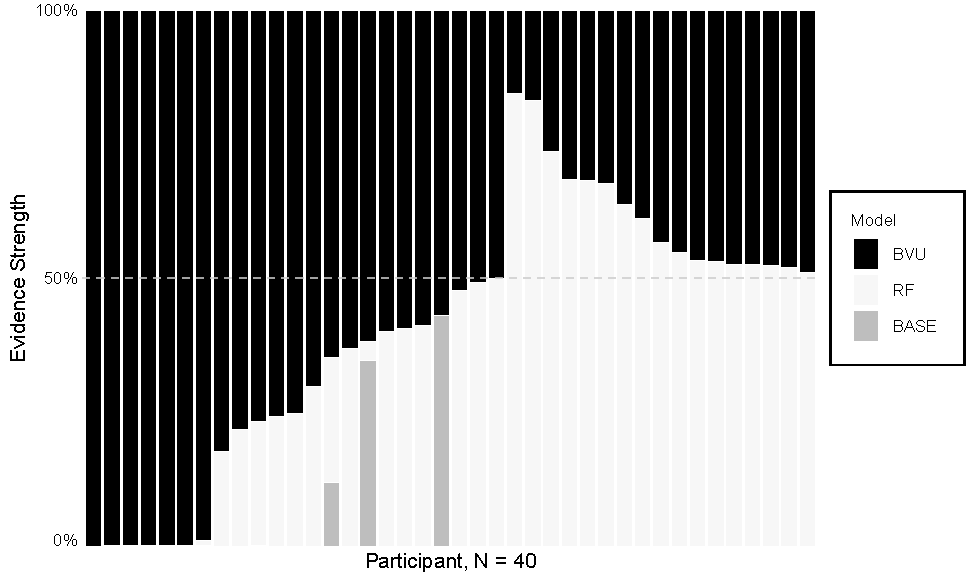
\includegraphics[width=.9\linewidth]{../figures/fig2_2-1} 

}

\caption{Evidence for the models for individual participants. \textit{RF}$=$ relative frequency model, \textit{BVU}$=$ Bayesian value updating model, \textit{BASE}$=$ Baseline model.}\label{fig:fig2_2}
\end{figure}

\added[id=jj]{
The fitted model parameters (Table \ref{tab:study1_parameter}) reveal that the power utility exponent did not differ markedly between the participants that were described by the Bayesian value updating strategy ($M_{\alpha}= 2.19$) and those described by a relative frequency strategy ($M_{\alpha}=2.15$), $\Delta$ $M = 0.02$ 95\% HDI $[-1.12$, $1.18]$, $\mathrm{BF}_{\textrm{01}} = 3.21$. Participants using the Bayesian strategy had, on average, a prior belief that gains occur with 45\% (gain prior $\theta_G = 0.91$; zero-outcome prior $\theta_0 = 1.09$). Also, their estimated learning rate $\delta$ was anti-conservative ($M_{\delta}=2.27$).
}

\begin{table}[tbp]

\begin{center}
\begin{threeparttable}

\caption{\label{tab:study1_parameter}Parameter Estimates of Winning Models, \textit{M (SD)}}

\begin{tabular}{lcccc}
\toprule
Winning Model & $\alpha$ & $\delta$ & $\theta_G$ & $\sigma$\\
\midrule
BVU (\textit{n}$=$23) & 2.19 (2.35) & 2.27 (3.39) & 0.91 (0.79) & 0.23 (0.22)\\
RF (\textit{n}$=$17) & 2.15 (1.45) & -- & -- & 0.15 (0.04)\\
\bottomrule
\addlinespace
\end{tabular}

\begin{tablenotes}[para]
\normalsize{\textit{Note.} \textit{BVU}$=$ Bayesian value updating model, \textit{RF}$=$ relative frequency model. Parameters denote: $\alpha=$ power utility exponent, $\theta_G$ gain prior, $\sigma$ standard deviation.}
\end{tablenotes}

\end{threeparttable}
\end{center}

\end{table}

\textit{Qualitative Model Fit.} Figure \ref{fig:fig5_2} plots the
qualitative model fit (best-fitting model predictions against observed
evaluations by participant). As in Study 1, the data are generally
well-described
\added[id=jj]{($M r\textsubscript{pred,obs} = 0.70$), except in four cases (participants s42, s47, s54, s67, with $r\textsubscript{pred,obs} < 0.40$)}
where the model must be rejected because of qualitative mis-fit.


\end{document}
